\section{MuhammadIqbalPanggabean(1174063)}
\subsection{Point Polyline dan Polygon}
\begin{enumerate}
	\item 
	\lstinputlisting{src/1/1174063/pyshp1.py}
	\begin{figure}[H]
		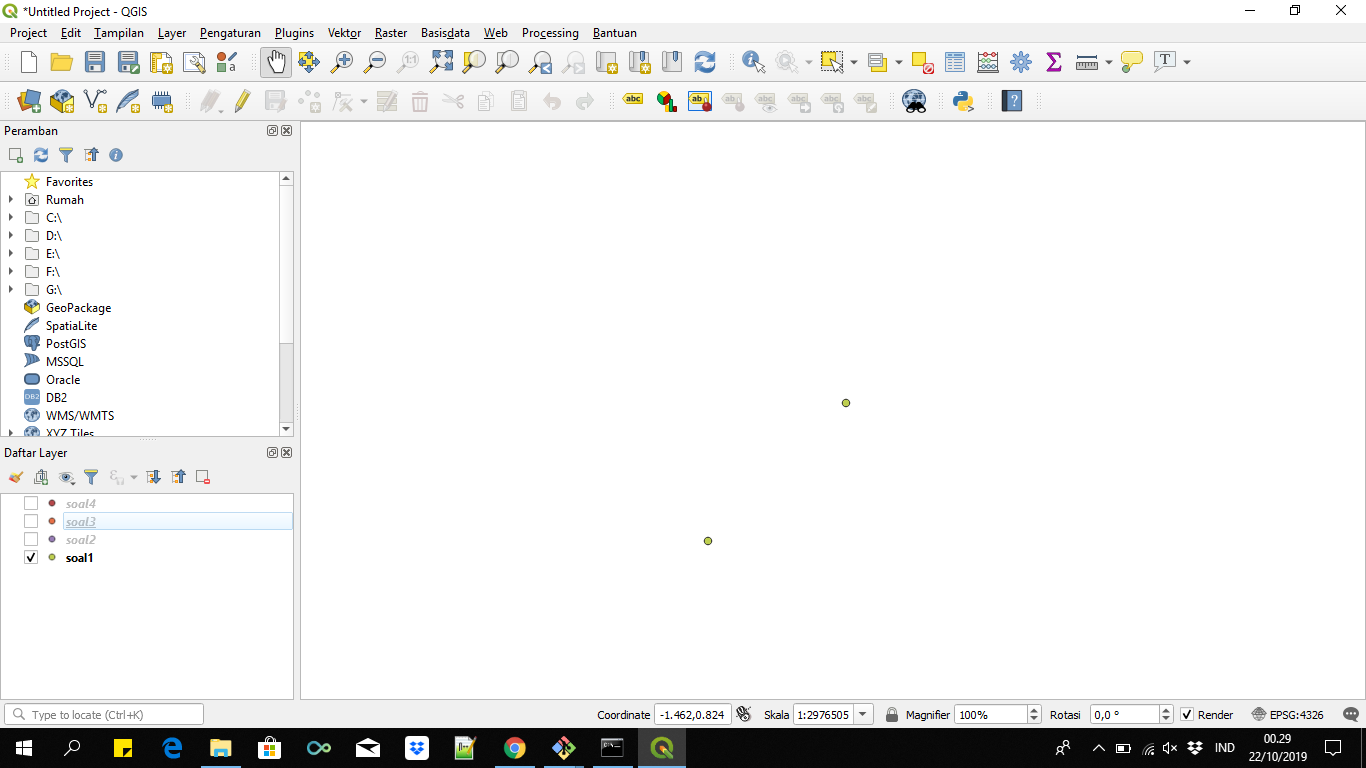
\includegraphics[width=12cm]{figures/1174063/1.PNG}
		\centering
		\caption{Point}
	\end{figure}
	
	\item 
	\lstinputlisting{src/1/1174063/pyshp2.py}
	\begin{figure}[H]
		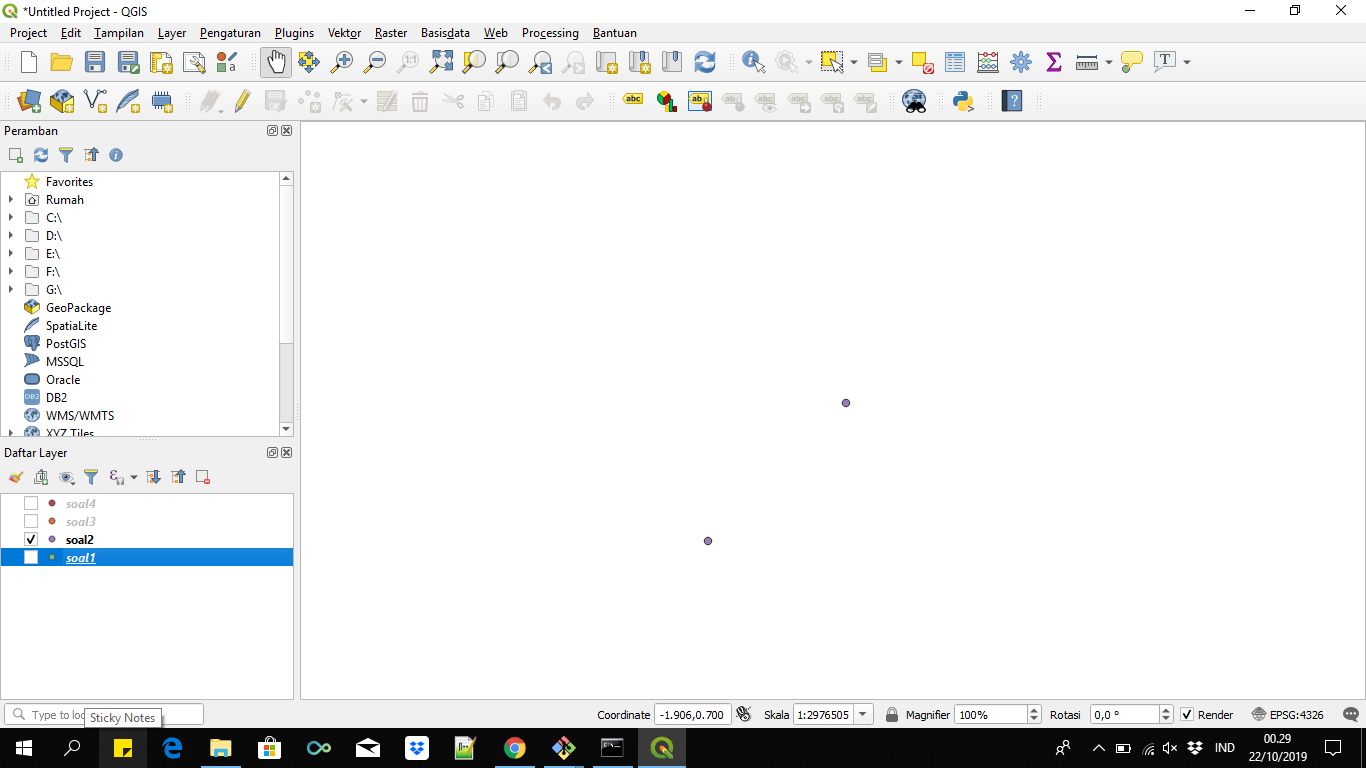
\includegraphics[width=12cm]{figures/1174063/2.PNG}
		\centering
		\caption{Point}
	\end{figure}
	
	\item 
	\lstinputlisting{src/1/1174063/pyshp3.py}
	\begin{figure}[H]
		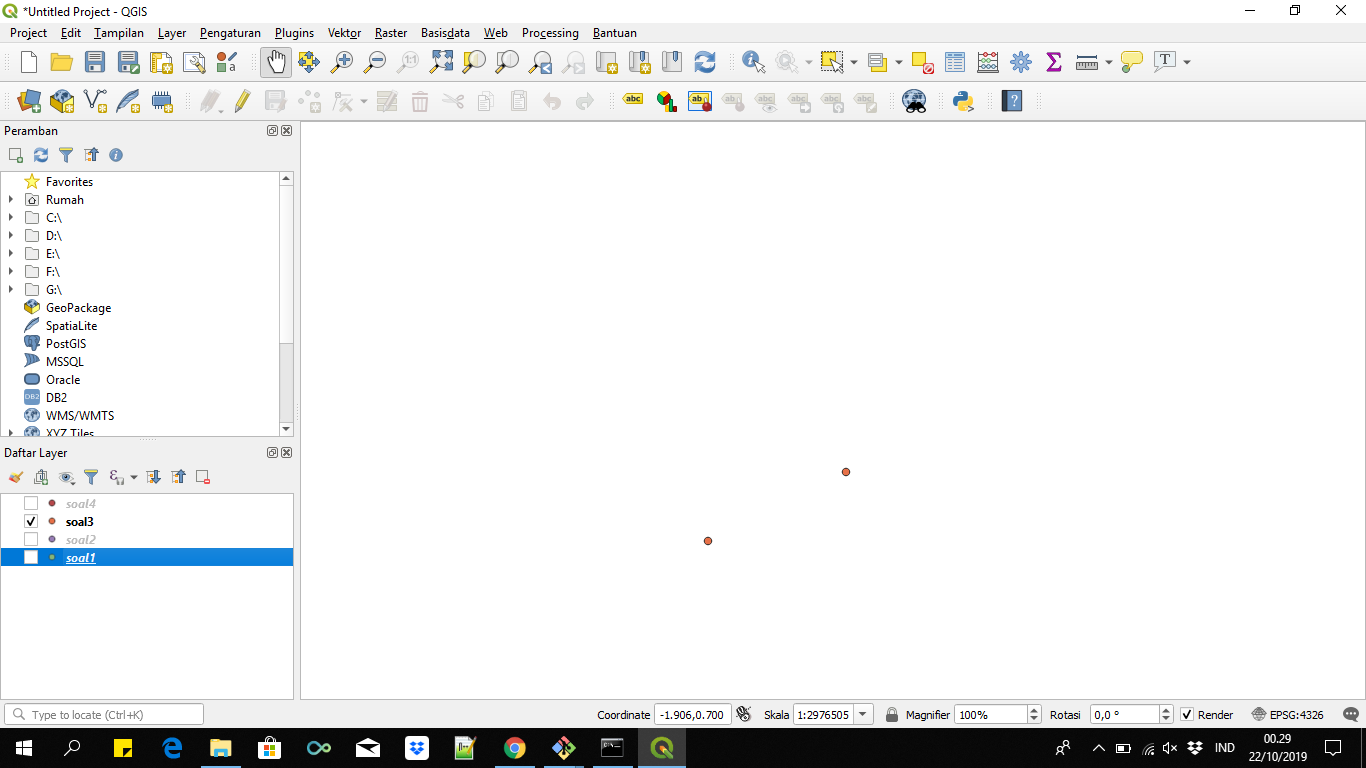
\includegraphics[width=12cm]{figures/1174063/3.PNG}
		\centering
		\caption{Point}
	\end{figure}
	
	\item 
	\lstinputlisting{src/1/1174063/pyshp4.py}
	\begin{figure}[H]
		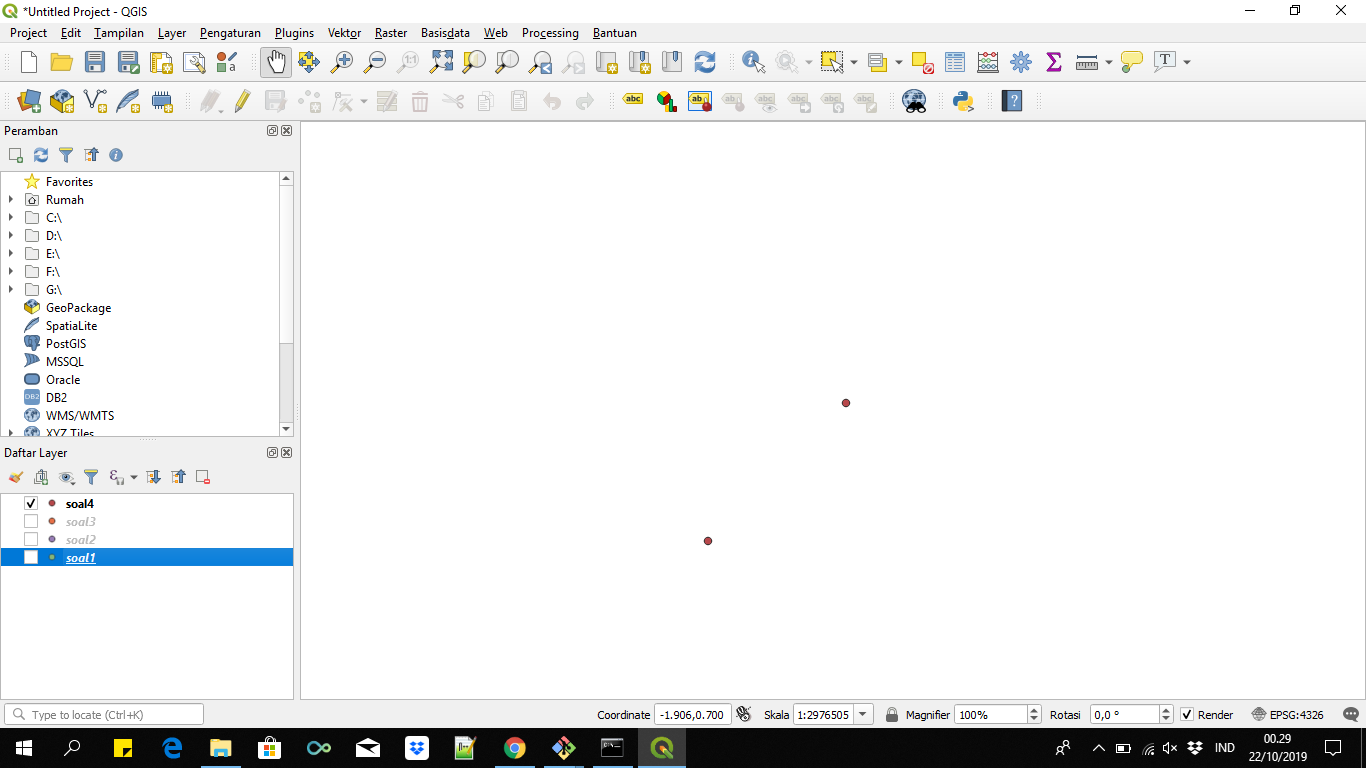
\includegraphics[width=12cm]{figures/1174063/4.PNG}
		\centering
		\caption{Point}
	\end{figure}
	
	\item 
	\lstinputlisting{src/1/1174063/pyshp5.py}
	\begin{figure}[H]
		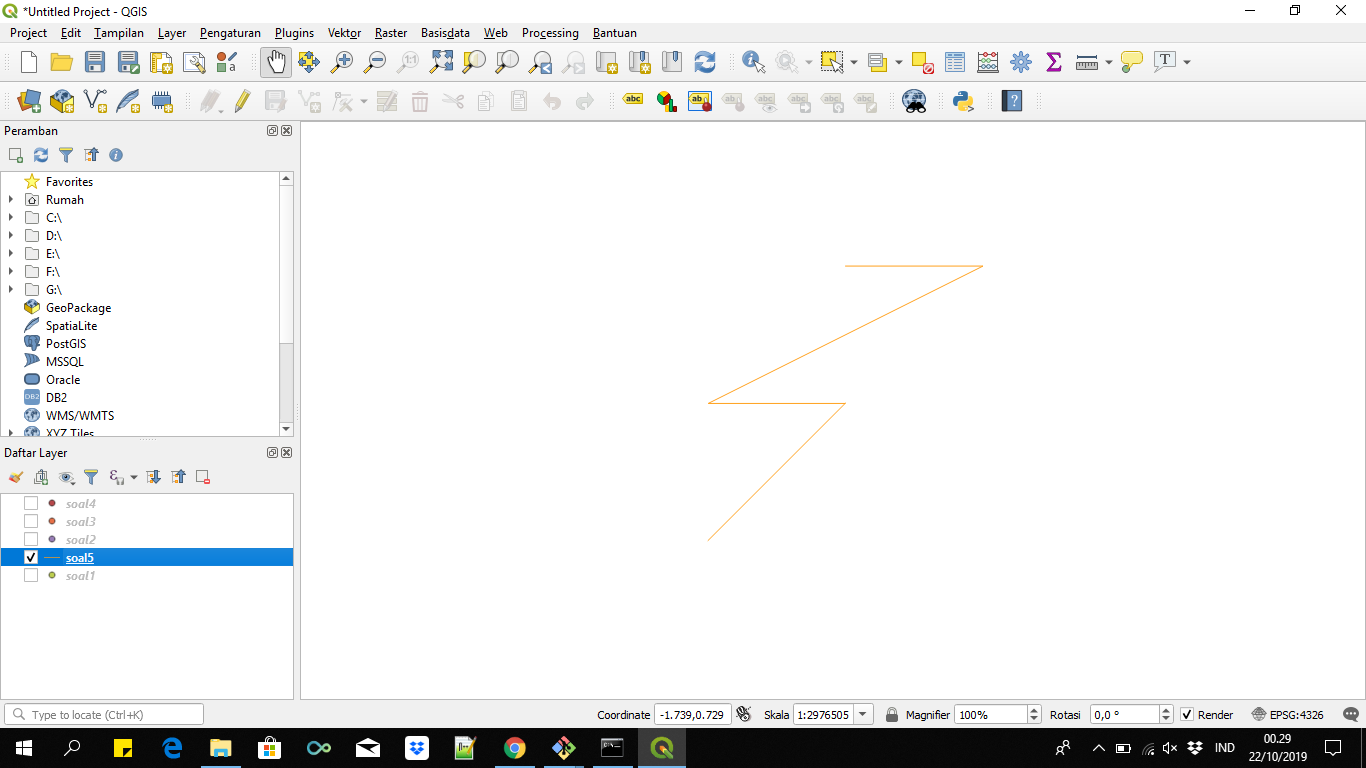
\includegraphics[width=12cm]{figures/1174063/5.PNG}
		\centering
		\caption{Polyline}
	\end{figure}
	
	\item 
	\lstinputlisting{src/1/1174063/pyshp6.py}
	\begin{figure}[H]
		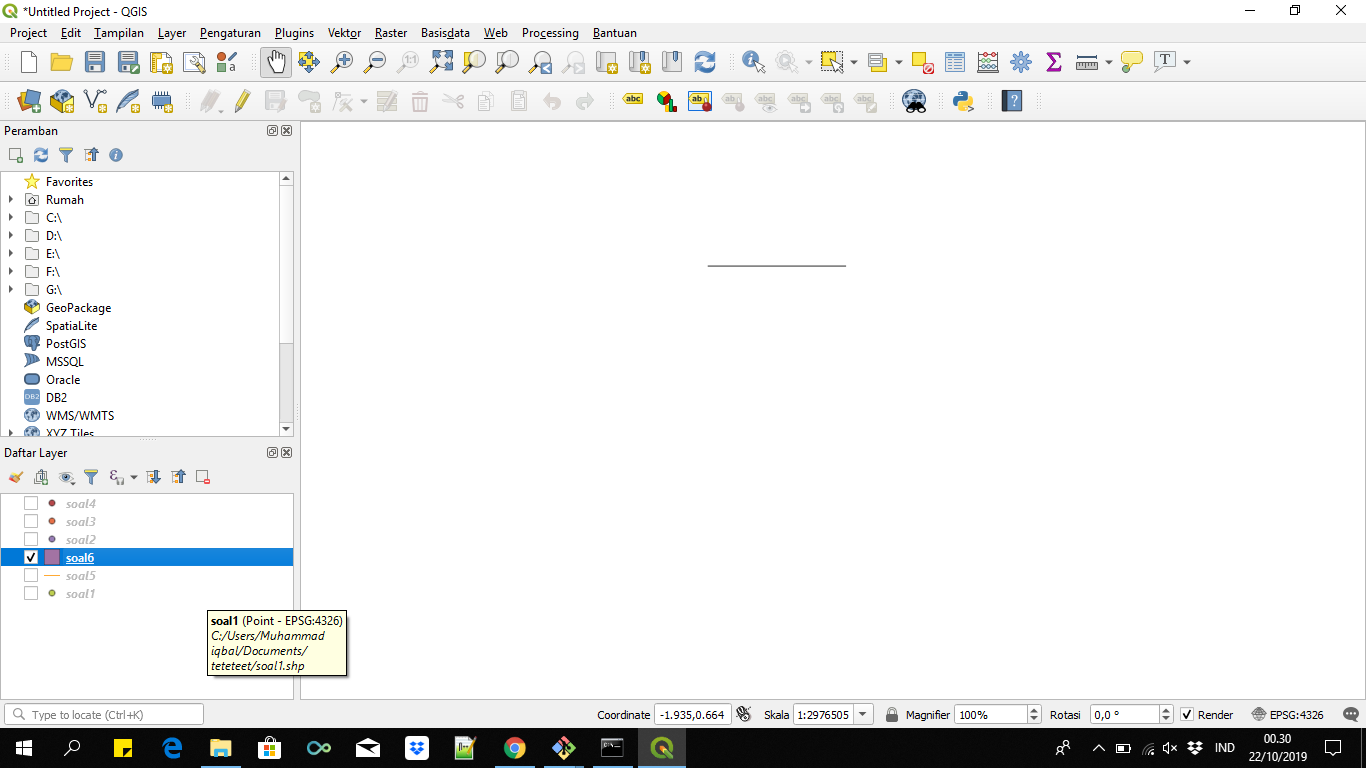
\includegraphics[width=12cm]{figures/1174063/6.PNG}
		\centering
		\caption{Poligon}
	\end{figure}
	
	\item 
	\lstinputlisting{src/1/1174063/pyshp7.py}
	\begin{figure}[H]
		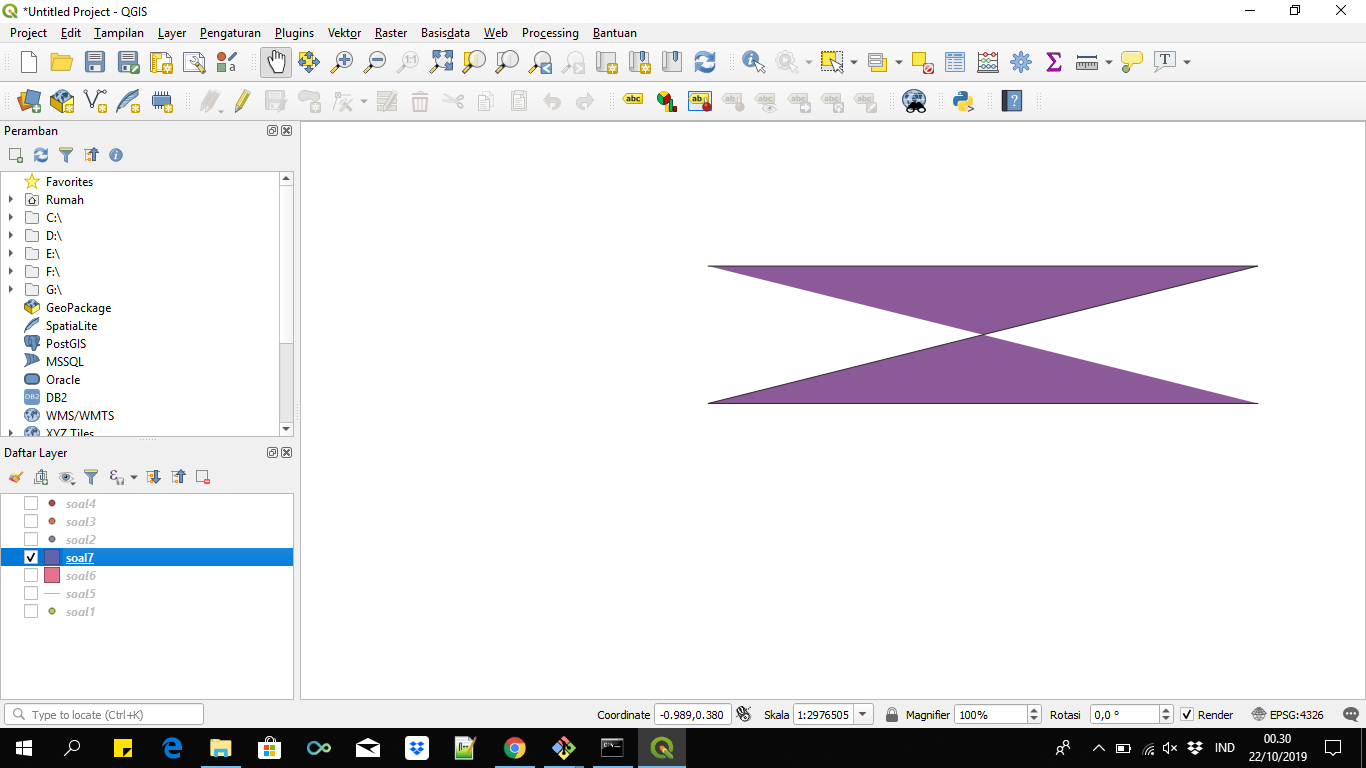
\includegraphics[width=12cm]{figures/1174063/7.PNG}
		\centering
		\caption{Polygon}
	\end{figure}
	
	\item 
	\lstinputlisting{src/1/1174063/pyshp8.py}
	\begin{figure}[H]
		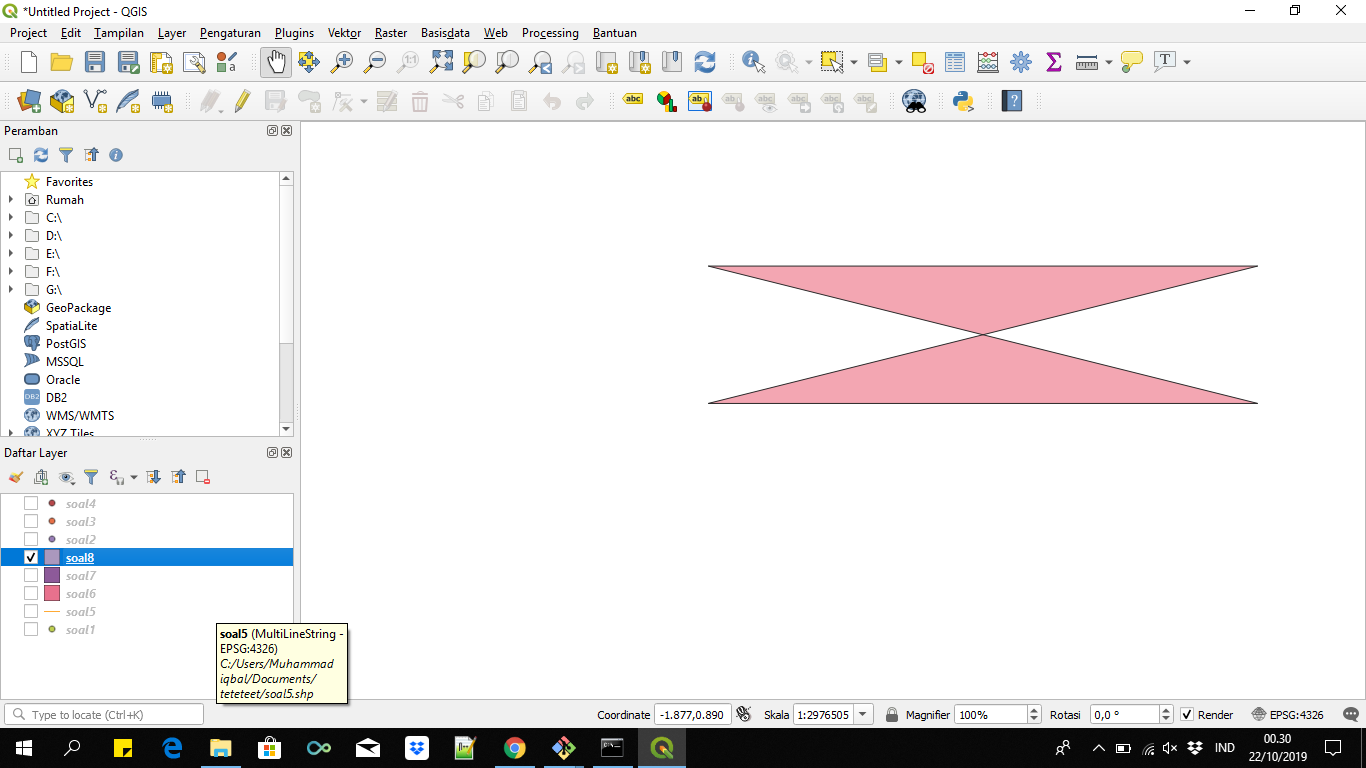
\includegraphics[width=12cm]{figures/1174063/8.PNG}
		\centering
		\caption{Polygon}
	\end{figure}
	
	\item 
	\lstinputlisting{src/1/1174063/pyshp9.py}
	\begin{figure}[H]
		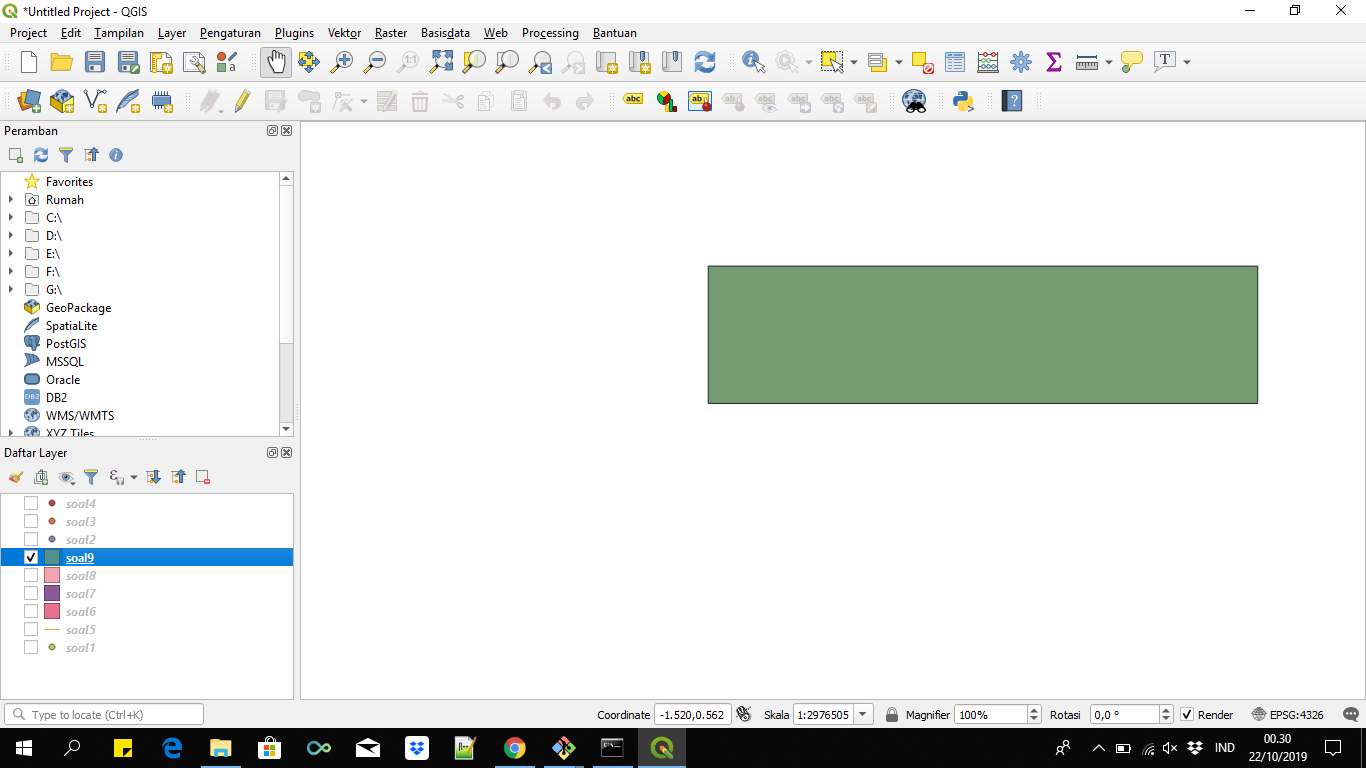
\includegraphics[width=12cm]{figures/1174063/9.PNG}
		\centering
		\caption{Polygon}
	\end{figure}
	
	\item 
	\lstinputlisting{src/1/1174063/pyshp10.py}
	\begin{figure}[H]
		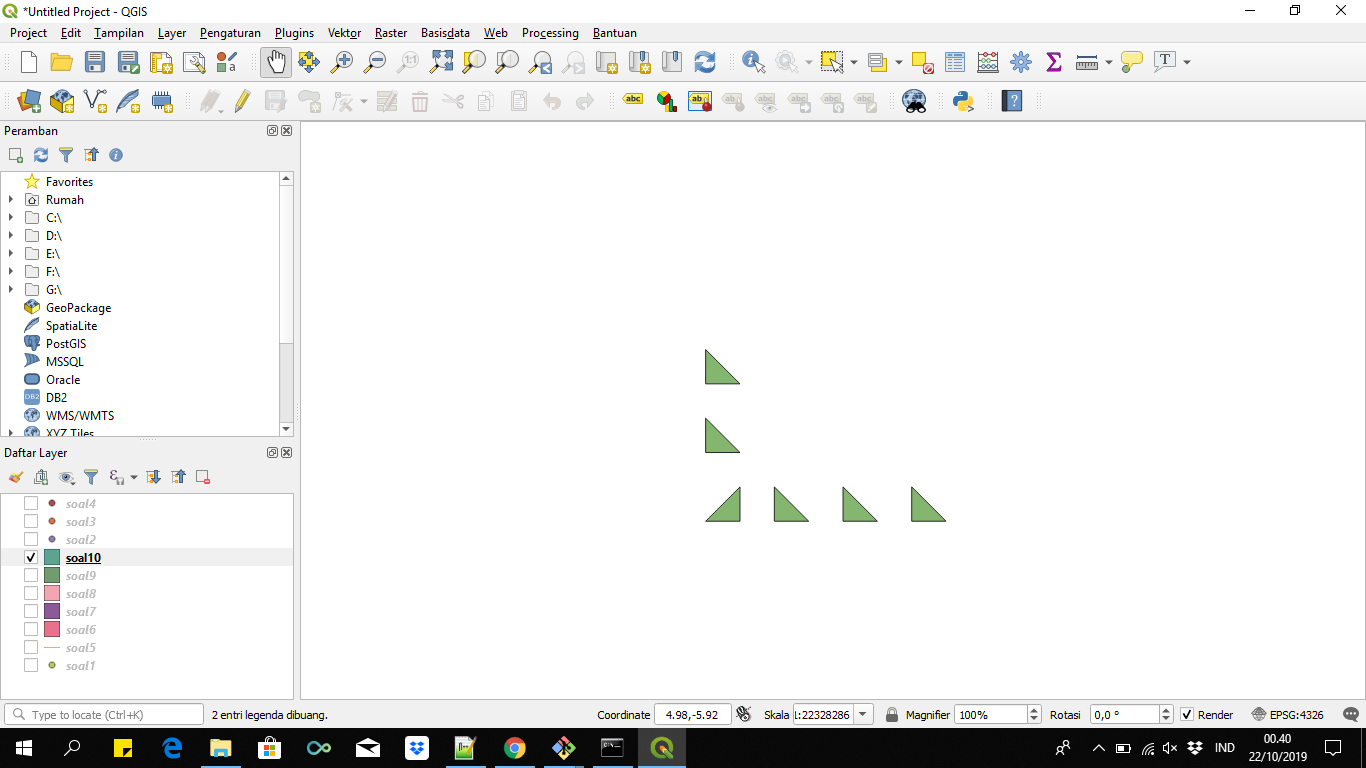
\includegraphics[width=12cm]{figures/1174063/10.PNG}
		\centering
		\caption{Hasil mod saya yaitu 2 jadi yang saya kerjakan Bujursangkar yang berjumlah 5, Polygon}
	\end{figure}	
\end{enumerate}

\subsection{Link}
\href{https://youtu.be/Yb9XchNG3qY}{Youtube! Dont Forget Subrettt!!}